\chapterimage{chapter_head_2.jpg} % Chapter heading image

\chapter{The College}
\addcontentsline{lof}{figure}{Chapter header \emph{Flag}: Photo credit to Sarah
White}

\section{History}

St Mary College of Winchester in Oxford, commonly known as New College, was
founded on the 26th~of November~1379. It was the seventh college, of those still in existence, to be founded at Oxford. Since 1400 it has been known as New College to distinguish it from the other college of St Mary (now Oriel College). The college was founded by the Bishop of Winchester, William of Wykeham, a churchman and administrator in the King's service, whose eventual wealth and power overshadow the humble obscurity of his origins. He established and endowed the college on a scale that, at the time, dwarfed any rival institution. The first part of college to be built was the Front or Old quad and the adjoining cloisters, which were constructed between the foundation and 1400. This was the first purpose-built quadrangle in Oxford and is unusual in that it has an oval lawn in the middle. Pre-dating this were the city walls, which are from the 13th Century: New College is obliged to maintain these and they form a pleasant backdrop to the college gardens.

In August~1651, New College was fortified by the Parliamentarian forces and the cloister was used for musketry training. In 1685, Monmouth's rebellion involved Robert Sewster, a fellow of the college, who commanded a company of university volunteers. These volunteers were mostly of New College and exercised in the Bowling Green.

The college was extended between 1681 and 1707 with the addition of the beautiful garden quad. At the end of the 19th Century the Holywell Quad, with the associated New Buildings was built to cope with expanding numbers in college. The Sacher building was built for graduate students in the sixties, making New College the first of the ancient colleges to build a common room especially for graduates. As of 2011, graduates are no longer housed in the Sacher building and are instead located all together in the lovely Weston Buildings. In 1979, the first women were admitted, after Governing Body initially began considering becoming co-residential in 1964, making it one of the first all male colleges to do so, but one of the latest to actually usher in this change.

\section{College motto}

The college's motto, created by William of Wykeham, is "Manners Makyth Man". The
motto was in many respects fairly revolutionary. Firstly, it was written in English, rather than Latin, which makes it very unusual in Oxford, and is especially revolutionary considering the college's age; even St Catherine's College, founded in 1965, has a Latin motto. Secondly, the motto makes a social statement. While it might initially seem to be suggesting that it is beneficial to have good manners, this does not really capture its full scope. What it really means is that it is not by birth, money, or property that an individual is defined, but by how he or she behaves towards other people.

\begin{figure}[htbp]
\centering
		\begin{minipage}{0.48\textwidth}
			\centering
                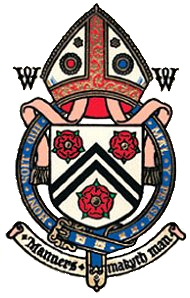
\includegraphics[width=.4\textwidth]{coat.png}
                \caption[]{William of
                Wykeham's coat of arms, including his motto}
                \label{fig:coat}
        \end{minipage}%
        \quad
        \begin{minipage}{0.48\textwidth}
        	\centering
                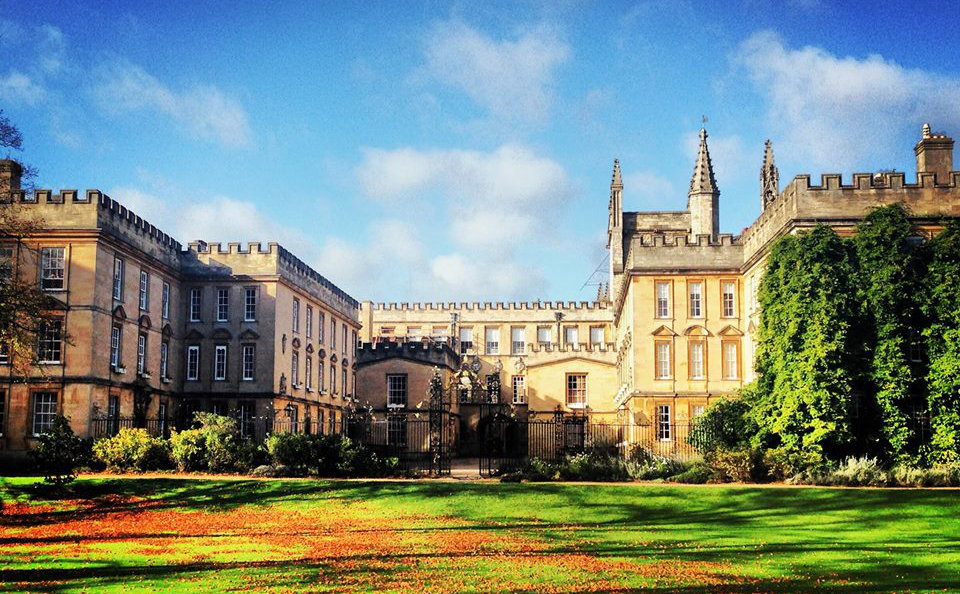
\includegraphics[width=\textwidth]{college.jpg}
                \caption[]{One of the nicer views
				of New College}
				\label{fig:college}
        \end{minipage}%
\end{figure}

\section{New College today}

New College is an intellectual community and one of the best-known colleges in
Oxford. New College has approximately 60~governing body fellows, 10~junior
fellows, 325 graduate students (109 freshers this year included),
420~undergraduates, an endowment of over \pounds160~million, a turnover of
\pounds13~million, and some of the most beautiful grounds and buildings in Oxford.

The college is governed, surprisingly, democratically, by the governing body
which consists of professorial fellows, tutorial fellows and a few others. New College has around 10~professorial fellows who hold university chairs. There are around 45~tutorial fellows who teach undergraduates in college as well as having university positions.

The primus inter pares is the Warden who serves as the figurehead of the college. Our new warden is Miles Young, who is the Chairman and CEO of one of the world's largest communications groups, Ogilvy and Mather.

The fellows and senior college officers make up the senior common room, or SCR. Physically this is located between the Front and Garden quads. They dine to near Michelin star standard, have a wine cellar of 40,000~bottles and have luxurious offices in the Old Quad buildings.

The MCR is made up of graduate students, people reading for second undergraduate degrees, visiting students, a few post-doctoral researchers without a college allegiance, and 4th year undergraduates in sciences, languages, and some other subjects. Graduate students are primarily taught by the university, but have college as a social base and to provide additional resources.

The JCR, or junior common room, is the undergraduate body. They are taught between college,
where they have regular tutorials (hour long sessions with their tutors, individually or in pairs), and the university where they have lectures and practicals. Admission of undergraduates is the responsibility of the colleges.

New College is particularly famous for its musical and cultural education. It houses a world class choir, with associated choir school, and the fellows have written many of the world's leading textbooks in the discipline. New College has just received planning permission for a new music building, adjacent to the Victorian Savile House in Mansfield Road. The building, designed by John McAslan and Partners, will offer three floors of accommodation: the top floor will contain two chamber music studios; the first floor, four practice rooms; and the ground floor, a large rehearsal room for opera and drama. Work will begin during the summer of 2015.
